\documentclass[t,xcolor=pst,dvips]{beamer}
\usepackage{pstricks,pst-grad,pst-text,pst-node,multido,pst-plot,calc,pst-3dplot}
%\usepackage{pstricks}
\mode<presentation>
\usetheme{Madrid}
% other themes: Warsaw, AnnArbor, Antibes, Bergen, Berkeley, Berlin, Boadilla, boxes, CambridgeUS, Copenhagen, Darmstadt, default, Dresden, Frankfurt, Goettingen,
% Hannover, Ilmenau, JuanLesPins, Luebeck, Madrid, Maloe, Marburg, Montpellier, PaloAlto, Pittsburg, Rochester, Singapore, Szeged, classic

\setbeamertemplate{navigation symbols}{\insertslidenavigationsymbol}

\usecolortheme{dolphin}
%\usecolortheme{seagull}
% color themes: albatross, beaver, beetle, crane, default, dolphin, dov, fly, lily, orchid, rose, seagull, seahorse, sidebartab, structure, whale, wolverine

%\usefonttheme{serif}
% font themes: default, professionalfonts, serif, structurebold, structureitalicserif, structuresmallcapsserif

% pdf is displayed in full screen mode automatically
%\hypersetup{pdfpagemode=FullScreen}

%\AtBeginSection[]
%{
%  \begin{frame}<beamer>
%    \frametitle{Outline}
%    \tableofcontents[currentsection,currentsubsection]
%  \end{frame}
%}



% define your own colours:
\definecolor{Red}{rgb}{1,0,0}
\definecolor{myblue}{rgb}{0,0,0.6}
\definecolor{Blue}{rgb}{0,0,1}
\definecolor{Green}{rgb}{0,1,0}
\definecolor{magenta}{rgb}{1,0,.6}
\definecolor{lightblue}{rgb}{0,.5,1}
\definecolor{lightpurple}{rgb}{.6,.4,1}
\definecolor{gold}{rgb}{.6,.5,0}
\definecolor{orange}{rgb}{1,0.4,0}
\definecolor{hotpink}{rgb}{1,0,0.5}
\definecolor{newcolor2}{rgb}{.5,.3,.5}
\definecolor{newcolor}{rgb}{0,.3,1}
\definecolor{newcolor3}{rgb}{1,0,.35}
\definecolor{darkgreen1}{rgb}{0, .35, 0}
\definecolor{darkgreen}{rgb}{0, .6, 0}
\definecolor{darkred}{rgb}{.75,0,0}
\definecolor{grayA}{rgb}{0.95,0.95,0.95}
\definecolor{grayB}{rgb}{0.98,0.98,0.98}

\xdefinecolor{olive}{cmyk}{0.64,0,0.95,0.4}
\xdefinecolor{purpleish}{cmyk}{0.75,0.75,0,0}

%\usepackage{beamerinnerthemerounded}
% inner themes include circles, default, inmargin, rectangles, rounded

%\usepackage{beamerouterthemesmoothbars}
% outer themes include default, infolines, miniframes, shadow, sidebar, smoothbars, smoothtree, split, tree

\useoutertheme[subsection=false]{smoothbars}

% to have the same footer on all slides
\setbeamertemplate{footline}[text line]{
\raisebox{3pt}{
\includegraphics[height=15pt]{su-long.eps}}\hfill 
\raisebox{5pt}{Math 207:  Statistics}\hfill 
\raisebox{5pt}{Controlled Experiments}\hfill
\raisebox{5pt}{\insertframenumber/\pageref{lastpage}}}
%\setbeamertemplate{footline}[text line]{} % or empty footer

% include packages
\usepackage{subfigure}
\usepackage{multicol}
\usepackage{amsmath}
\usepackage{epsfig}
\usepackage{graphicx}
%\usepackage[all,knot]{xy}
%\xyoption{arc}
\usepackage{url}
\usepackage{multimedia}
\usepackage{hyperref}
\usepackage{setspace}

\title{Math 207:  Statistics}
\subtitle{Controlled Experiments}
\author{Dr.~Ralph Wojtowicz}
\institute{Mathematics Department\\ Shepherd University}
%\date{\scriptsize 22 August 2011}


\begin{document}

%\frame[plain]{
%	\titlepage
%}

\begin{frame}[plain]

\begin{center}
\begin{pspicture}(-6,-7)(6,2)
\psframe[linewidth=0.02,linecolor=gray](-6.2,-7)(6.2,2.2)
\psframe[linewidth=0.02,linecolor=gray](-6.15,-6.95)(6.15,2.15)
\rput(0,1.2){\color{myblue}\large Math 207:  Statistics}
\rput(0,0.2){\color{myblue}Controlled Experiments}
%
\psframe[linewidth=0.02,fillstyle=solid,fillcolor=grayA](-2,-3)(2,-1)
  \rput[tl](-1.9,-1.1){\tiny Population (parameters)}
\psframe[linewidth=0.02,fillstyle=solid,fillcolor=grayB](-0.25,-2.75)(1.75,-2)
  \rput[tl](-0.15,-2.1){\tiny Sample (statistics)}
%
\rput(0,-4.2){\scriptsize Dr.~Ralph Wojtowicz}
\rput(0,-4.7){\scriptsize Mathematics Department}
\rput(0,-5.5){
\includegraphics[height=1cm]{su-long.eps}}
%
%\rput(0,-6.5){\scriptsize 22 August 2011}
\end{pspicture}
\end{center}

\end{frame}


\addtocounter{page}{-1}
\addtocounter{framenumber}{-1}
%\frame{\tableofcontents}

\section{Salk Vaccine}
\subsection{Polio}
\begin{frame}[t]\frametitle{Polio}
\label{polio}

\begin{itemize}
\item Viral infectious disease: victims are typically children
\item Can effect nervous system causing muscle weakness or paralysis 
\item Most cases cause no symptoms but can spread the disease
\item Major epidemics across the world between 1910 and 1956
\item Vaccines discovered in 1950s have made polio rare in most countries
\end{itemize}

\begin{center}
{\small\setlength{\tabcolsep}{0.2in}\begin{tabular}{ccc}
%{\includegraphics[height=1.1in]{polio_victim.eps}}
{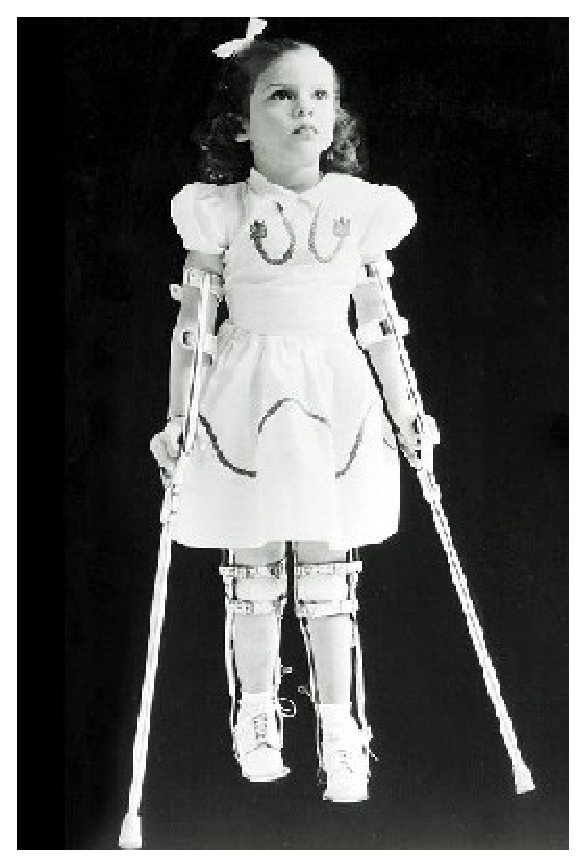
\includegraphics[height=1.1in]{polioDM.eps}}
& %\hspace{.4in}
\raisebox{-0.1in}{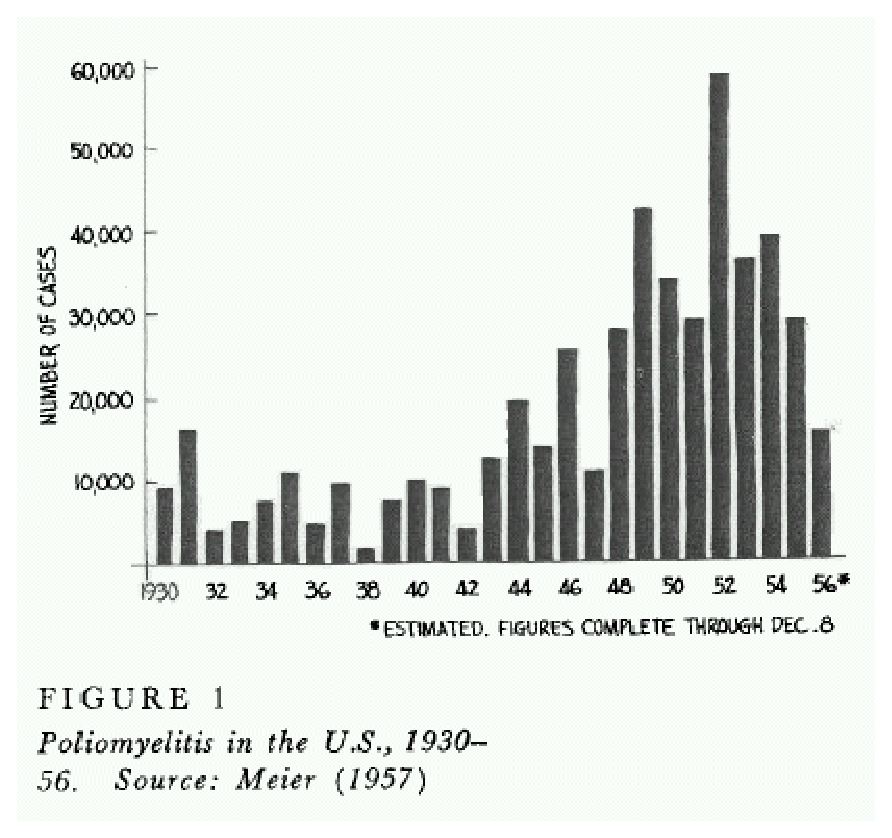
\includegraphics[height=1.2in,  bb=0 75 412 386, clip]{polioStatistics.eps}}
& %\hspace{.4in}
{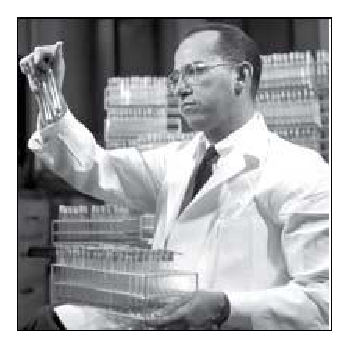
\includegraphics[height=1.1in]{jonas-salk.eps}}\\
Polio Victim & Infection Statistics & Jonas Salk
\end{tabular}}
\end{center}

\end{frame}

\subsection{Vaccine Trial Design Proposals}
\begin{frame}[t]\frametitle{Vaccine Trial Design Proposals}
{\small 

\begin{itemize}
\item 1954: Salk vaccine ready to tested outside the laboratory
\item Public Health Service and National Foundation for Infantile Paralysis (NFIP) 
  designed the experiments
\item Trials involved 2,000,000 grade 1--3 children in school districts across the US
   \begin{itemize}
      \item 500,000 vaccinated
      \item 1,000,000 deliberately left unvaccinated, as controls
      \item 500,000 refused vaccination
   \end{itemize}
\item Vaccine Trial Design Proposals
   \begin{itemize}
   \item Vaccinate a large number of children in 1954 and compare the polio incidence rate to that in 1953
          (not used:  see the graph on slide~\pageref{polio})
   \item Vaccinate all grade 2 children whose parents consent; leave children in grades 1 and 3 as controls
          (used in some school districts)
   \item From the set $X$ of children whose parents consent, randomly select some for vaccination; leave
         others in $X$ as controls
         (used in some school districts)
   \end{itemize}
\end{itemize}}

\end{frame}

\subsection{Complicating Factors}
\begin{frame}[t]\frametitle{Complicating Factors}
{\small
Challenges
\begin{itemize}
\item Children could not be vaccinated without parental consent
\item Higher-income parents were more likely to give consent
\item Children of higher-income families were more vulnerable to polio
\item Some cases are difficult to diagnose
\item Infection rate can vary from grade to grade
\end{itemize}
\medskip

Solutions
\begin{itemize}
\item Treatment and control groups should be as similar as possible, except for the treatment.
\item Use randomness rather than human judgment to assign subjects to groups and avoid bias.
\end{itemize}}
\end{frame}
 
\subsection{Trial Results}
\begin{frame}[t]\frametitle{Trial Results}
{\ }\vspace{-20pt}
\begin{center}
{\footnotesize
\begin{tabular}{cc}
Randomized controlled          & \\
double-blind experiment        & NFIP study\\
   \begin{tabular}{lcc}\hline
                 & Size      & Rate${}^*$\vphantom{\LARGE Y}\\
      \color{darkgreen}Treatment  & \color{darkgreen}200,000   & {\color{blue}\textbf{28}}\\
      \color{darkgreen}Control    & \color{darkgreen}200,000   & {\color{blue}\textbf{71}}\\
      No consent & 350,000   & 46\\
   \end{tabular}
&
   \begin{tabular}{lcc}
\hline
                 & Size        &  Rate${}^*$\vphantom{\LARGE Y}\\
      \color{darkgreen}Grade 2 (vaccine)\hfill        & \color{darkgreen}225,000 & 25\\
      \color{gray}Grades 1 and 3 (control)        & \color{gray}725,000 & {\color{red}\textbf{54}}\\
      Grade 2 (no consent)\hfill     & 125,000 & {\color{red}\textbf{44}}\\
   \end{tabular}
\end{tabular}}\vspace{-2pt}
\end{center}
{\scriptsize ${}^*$Rate is number of cases per 100,000 subjects.
  $\mbox{\color{darkgreen}Green}=\mbox{consent}$  $\mbox{\color{gray}Gray}=\mbox{consent}+\mbox{no consent}$}

{\small\begin{itemize}
\item Blue values demonstrate vaccine effectiveness: Could the 
  ${\color{blue}\textbf{71}}\to {\color{blue}\textbf{28}}$ difference be due to the 50/50 
  selection chance?
\item Red values demonstrate that the NFIP study treatment and control groups differed 
  in their vulnerability %(only consenting families in treatment group)
\item ${\color{blue}\textbf{71}}\to {\color{blue}\textbf{28}}$ 
    vs ${\color{red}\textbf{54}}\to 25$ shows bias in NFIP study due to confounding
\item Average of blue values (50) differs from 46: children of consenting parents 
  were more vulnerable
%\item Compre 46 to 44
\end{itemize}}
%Exercises:  3 on page 25, 
\end{frame}

\subsection{Vaccine Trial Concepts}
\begin{frame}[t]\frametitle{Vaccine Trial Concepts}

{\small\begin{itemize}
\item Treatment group: children  selected for vaccination
\item Control group: children  selected not to be vaccinated
\item Comparison:  estimate the effectiveness of the vaccine by 
  comparing the infection rates (responses) of the two groups
\item Double-blind:  neither the subjects nor the medical examiners knew who was in the treatment group and 
who was in the control group
\item Placebo: children in the control group were given an injection of salt water
\item Confounding:  a difference (such as family income)
   between the treatment and control groups --- other than the treatment ---
   which affects the responses being studied.
%some factor, such as family income, other than treatment can impact
%  the trial results
\item Random:  chosen without regard to any characteristics of the 
  individual members of the population so that each has an equal chance of being 
  selected.
\end{itemize}}
\end{frame}


\section{Portacaval Shunt}

\subsection{Cirrhosis of the Liver}

\begin{frame}[t]\frametitle{Cirrhosis of the Liver}
{\small
\begin{itemize}
\item Cirrhosis of the liver:  multiple causes including alcoholism and hepatitis B/C
\item Without a liver transplant, outcomes are usually poor
\item A possible complication is internal bleeding that results in death
\item Surgery to redirect blood flow through a portacaval shunt has been studied as a potential treatment
\item The procedure is long and hazardous
\item Numerous studies have been conducted to asses the value of the surgery
   \begin{itemize}
      \item 32 without controls
      \item 15 with non-randomized controls
      \item {\color{white}0}4 with randomized controls
   \end{itemize}
\end{itemize}

}
\end{frame}

\subsection{Results}

\begin{frame}[t]\frametitle{Results of Studies}
{\small
\begin{itemize}
\item Of the 51 studies conducted to assess the effect of the surgery:
   \begin{itemize}
      \item 75\% of studies without controls were markedly enthusiastic about shunt
      \item 67\% of non-randomized studies were markedly enthusiastic
      \item {\color{white}0}0\% of randomized studies were markedly enthusiastic
   \end{itemize}
%\item The poorly studies exaggerated the value of the surgery
\end{itemize}
}
%
{\footnotesize
\begin{center}
\begin{tabular}{lccc}
&&\hspace{-0.45in} Degree of enthusiasm\span\\[2pt]
Design & Marked & Moderate & None\\[2pt]\hline
No controls                  & 24 & 7 & 1\vphantom{\LARGE Y}\\
Controls, but not randomized & 10 & 3 & 2\\
Randomized controlled        & \hphantom{0}0 & 1 & 3
\end{tabular}
\end{center}}
{\small
\begin{itemize}
\item Three-year survival rates show that subjects selected for surgery in the non-randomized studies
   were healthier than the controls
\end{itemize}}
%
{\footnotesize
\begin{center}
\begin{tabular}{lcc}
         & Randomized & Not randomized\\[2pt]\hline
Surgery  & 60\%        & 60\%  \vphantom{\LARGE Y}\\
Controls & 60\%        & 45\%
\end{tabular}
\end{center}}

\end{frame}

\section{Historical Controls}

\subsection{Coronary Artery Disease Therapies}
\begin{frame}\frametitle{Coronary Artery Disease Therapies}

{\small 
\begin{itemize}
\item Randomized controlled experiments can be hard to do.
\item Treatment groups are often compared to historical rather than contemporaneous controls.
\end{itemize}}\vspace{-10pt}
{\footnotesize
\begin{center}
\begin{tabular}{lccrc}
        & Randomized\span & Historically\span\\
Therapy & controlled\span & controlled\span\\[2pt]\hline
                         & $+$ & $-$       & $+$ & $-$\\
Coronary bypass surgery  & 1 & 7 & 16 & 5\\
5-FU                     & 0 & 5 & 2 & 0\\
BCG                      & 2 & 2 & 4 & 0\\
DES                      & 0 & 3 & 5 & 0
\end{tabular}\vspace{-3pt}
\end{center}
}

{\small 
\begin{itemize}
\item Three-year survival rates for surgery patients and controls show that 
  that the treatment and historical control groups differed: patients selected for surgery were 
  healthier.
\end{itemize}}\vspace{-10pt}
{\footnotesize
\begin{center}
\begin{tabular}{lcc}
         & Randomized & Historical\\[2pt]\hline
Surgery  & 87.6\%     & 90.9\%    \\
Controls & 83.2\%     & 71.1\%
\end{tabular}
\end{center}}
\end{frame}

\section{Experiments}
\subsection{Experiments}
\begin{frame}[t]\frametitle{Controlled Experiments vs Observational Studies}
{\small 
\begin{itemize}
\item \textbf{Controlled experiment}: Investigators decide who will be in the treatment group and who will 
  be in the control group
     \begin{itemize}
     \item Example:  Salk vaccine trials discussed in Chapter 1
     \item Example:  Coronary Drug Project discussed in Section 2.2
     \item The control and treatment populations are similar --- except in the application of treatment
     \end{itemize}
\item \textbf{Observational study}: Subjects assign themselves to the groups
     \begin{itemize}
     \item Example:  Smoking studies
%     \item The two populations differ in ways other than the treatment
     \item \textbf{Association} between treatment and outcome is circumstantial evidence for causation.    
     \item Association does not prove causation.  \textbf{Confounding} factors may exist.
     \item Observational studies can be powerful tools but can also be misleading.% due to confounding.  
       \begin{itemize}
         \item Were the control and treatment groups similar?
         \item Did the two populations differ in ways other than the treatment?
       \end{itemize}
     \item Technique:  compare small, more homogeneous groups (e.g.,~age, sex)
     \end{itemize}
\end{itemize}}
\end{frame}

\subsection[Studies]{Classification of Studies}
\begin{frame}[t]\frametitle{Classification of Studies}
{\footnotesize
\begin{center}
\begin{pspicture}(0,0)(7,4.8)
\psset{xunit=1.4,yunit=1.2,nodesep=2pt}
\rput(4,4){\rnode{Studies}{Studies}}
\rput(5,3){\rnode{NoControls}{No Controls}}
\rput(3,3){\rnode{Controls}{Controls}}
\rput(4,2){\rnode{Historical}{Historical}}
\rput(2,2){\rnode{Contemporaneous}{Contemporaneous}}
\rput(1,1){\rnode{Controlled}{\begin{tabular}{c}Controlled\\ Experiment\end{tabular}}}
\rput(3,1){\rnode{Observational}{\begin{tabular}{c}Observational\\ Studies\end{tabular}}}
\rput(0,0){\rnode{Randomized}{Randomized}}
\rput(2,0){\rnode{NotRandomized}{Not Randomized}}
\ncline{Studies}{Controls}\ncline{Studies}{NoControls}
\ncline{Controls}{Contemporaneous}\ncline{Controls}{Historical}
\ncline{Contemporaneous}{Controlled}\ncline{Contemporaneous}{Observational}
\ncline{Controlled}{Randomized}\ncline{Controlled}{NotRandomized}
%\psframebox(0,0)(4,4)
\end{pspicture}
\end{center}}
\bigskip

\end{frame}

\section{Clofibrate}
\subsection{Clofibrate}
\begin{frame}[t]\frametitle{Clofibrate}
{\small
\begin{itemize}
\item Coronary Drug Project:  randomized, controlled double-blind experiment 
  (placebo $=$ lactose) to evaluate heart attack prevention drugs
\item 8,341 patients followed for five years (5,552 got treatment, 2,789 controls)
\item Clofibrate:  a cholesterol reduction drug evaluated in the study
\item Comparing 20\% to 21\% shows that clofibrate did not save lives.
\item Many subjects did not take their medicine (non-adherers).
\item Compare 15\% to 15\% (not to 21\% or 25\%)  to control for adherence.
\end{itemize}}\vspace{-8pt}
%
\begin{center}
{\newcommand{\Z}{\hphantom{0,}}\footnotesize\begin{tabular}{lcccc}
& \Z\Z Clofibrate\span  & \Z\Z Placebo\span\\[2pt]\hline
         & Number & Deaths & Number & Deaths\vphantom{\Large Y}\\
Adherers     & \Z708 & 15\% & 1,813 & 15\%\\
Non-adherers & \Z357 & 25\% & \Z882 & 28\%\\
Total group  & 1,103 & 20\% & 2,789 & 21\%
\end{tabular}} \vspace{-8pt}
\end{center}
{\small
\begin{itemize}
\item Conclusions:  (i) Clofibrate does not have an effect.  (ii) Adherers are different from non-adherers.
\end{itemize}}
\end{frame}

\section{Confounding}
\subsection{Confounding Factors and Associations}
\begin{frame}[t]\frametitle{Confounding Factors and Associations}
{\small
\begin{itemize}
\item Pellagra:  Among many associations between the 18${}^{th}$ century disease and other factors, lack of niacin
  was found to be the underlying cause.
\item Cervical Cancer and Circumcision: Human papilloma virus was found to be the underlying cause
  and explained differences in cancer rates between particular populations in the 1950s.
\item Ultrasound and low birthweight:  The confounding factor of problem pregnancy was found to 
  explain an association between ultrasound and low birthweight.  Randomized controlled experiments 
  showed that ultrasounds may be protective.
\item The Samaritans and Suicide:  A confounding factor explained an association between the 
  expansion of a volunteer welfare organization and a decrease in the English suicide rate 
  in 1964--1970.
\end{itemize}
}
\end{frame}

\subsection{Confounding}
\begin{frame}[t]\frametitle{Confounding}

{\small
\begin{itemize}
\item \textbf{Confounding}:  A difference between the treatment and control groups --- other than the treatment ---
   that affects the responses being studied
\item Confounders must be assocated with both:
   \begin{itemize} 
     \item The disease/outcome and 
     \item The exposure/treatment.
   \end{itemize}
\item Hidden confounders are a major problem in observational studies.
\item Examples:
   \begin{itemize}
   \item NFIP polio vaccine study:  family income
   \item Portacaval shunt studies:  health of patients selected for surgery
   \item Coronary bypass surgery studies:  health of patients selected for surgery
   \item Cervical cancer study: sexual activity
   \end{itemize}
\end{itemize}}
\end{frame}


\section{Simplson Paradox}
\subsection{Sex Bias in Graduate Admissions}
\begin{frame}[t]\frametitle{}
{\small
\begin{itemize}
\item Observational study on sex bias in admissions at UC, Berkeley in 1973
   \begin{itemize}
   \item 44\% of 8,442 male applicants were admitted
   \item 35\% of 4,321 female applicants were admitted
   \end{itemize}
\item Compare admissions to the six largest majors:\vspace{-9pt}
\end{itemize}}

{\footnotesize
\begin{center}
\newcommand{\Z}{\hphantom{0}}
\begin{tabular}{ccccc}
      & \Z\Z\Z\Z\Z\Z Men\span   & \Z\Z\Z\Z\Z Women\span\\[3pt]
      & Number of  & Percent  & Number of  & Percent\\
Major & Applicants & Admitted & Applicants & Admitted\\[2pt]\hline
A     & {\color{red}\textbf{825}}        
                   & {\color{red}\textbf{62}}       
                              & {\color{red}\textbf{108}}        
                                           & {\color{red}\textbf{82}}\vphantom{\large Y}\\
B     & 560        & 63       & 25         & 68\\
C     & 325        & 37       & 593        & 34\\
D     & 417        & 33       & 375        & 35\\
E     & {\color{blue}\textbf{191}}        
                   & {\color{blue}\textbf{28}}       
                              & {\color{blue}\textbf{393}}        
                                           & {\color{blue}\textbf{24}}\\
F     & 373        & \Z6      & 341        & \Z7
\end{tabular}\vspace{-16pt}
\end{center}}
%
{\small
\begin{itemize}
\item Major A:  Less selective but few women and many men applied
\item Major E:  Highly-selective but many women and few men applied
\item Simpson's paradox:  Relationships between percentages in subgroups can 
  be reversed when the subgroups are combined.
\end{itemize}}
\label{lastpage}
\end{frame}


\end{document} 
